%\documentclass[12pt, preprint,numberedappendix]{emulateapj}
%\documentclass[12pt, preprint]{aastex}
%\documentclass[apj]{emulateapj}
\documentclass[12pt, letterpaper]{article}

%\newcommand\submitms{n}		% set to y to follow AAS ``ms'' names, etc.
%\newcommand\bibinc{n}		% set to y if bib pasted in .tex, set to n to use bibtex


%\usepackage{pdfsync}
%\usepackage{subeqnarray}
\usepackage[top=0.8in, bottom=0.7in, left=1in, right=1in]{geometry}
\usepackage{natbib}
\usepackage{color}
\usepackage{graphicx}
\usepackage{fancyhdr}
\usepackage[T1]{fontenc}
\usepackage{titling}
\usepackage{sectsty}
\usepackage{sidecap}
\usepackage{placeins}
\usepackage{indentfirst}
\setlength{\droptitle}{-7em}
\setlength{\abovecaptionskip}{-0.4ex}
\setlength{\belowcaptionskip}{-0.4ex}
%\pagenumbering{gobble}
\pagestyle{fancy}
\lhead{Ana-Maria Piso}
\rhead{UC President's Postdoctoral Fellowship Research Statement}
\date{}
%\rhead{\thepage}


%\bibliographystyle{apj}

\title{\Large UC President's Postdoctoral Fellowship Research Statement: \\
\textbf{How Unique is the Solar System? Planetary Luminosities as Fingerprints for the Origins and Properties of Exoplanets}}
\author{Dr. Ana-Maria Piso}

%\newenvironment{packed_item}{
%\begin{itemize}
%  \setlength{\itemsep}{1pt}
%  \setlength{\parskip}{0pt}
%  \setlength{\parsep}{0pt}
%}{\end{itemize}}

\begin{document}
\maketitle

%\slugcomment{Draft Modified \today}

\vspace{-0.9cm}


Within the last two decades, more than one thousand extrasolar planets (exoplanets) have been discovered [1]. Their diversity in terms of mass, radius, location and composition [2] provides an exciting field of research, with the eventual goal of finding planets that are similar to our own Earth and that may sustain life. The advent of the Kepler Space Telescope has resulted in an exponential increase in the number of exoplanets detected via the transit method. As shown in Figure 1, a large fraction of the planets detected by Kepler are the so-called ``Super Earths'' or ``Mini Neptunes'', planets with masses between 1 and 10 times that of the Earth, and which are likely to contain some of their mass in a gaseous envelope. The majority of these detected Super Earths are very close to their host stars, with smaller orbital periods than the Earth. These features imply that Super Earths are not Solar System analogs. At the same time, they are ubiquitously found and predicted to be the most common types of exoplanets known to date [3], which makes understanding their ages, formation and properties particularly relevant. Observational techniques such as gravitational microlensing and direct imaging have extended the orbital range at which planets have been detected from just outside the Earth's orbit to tens and even hundreds of astronomical units. As demonstrated in Figure 2, however, most of these planets have Jupiter-like masses; true Uranus or Neptune analogs have yet to be detected. Are they indeed rare at these large distances, or just not bright or young enough to be detected? The Gemini Planet Imager (GPI) exoplanet survey will be key in improving our knowledge on this matter. GPI is a direct imaging survey that aims to observe very young, bright planets. As planets become less bright with increasing age, GPI might thus be able to detect lower mass planets that are just at the end stages of their formation. A theoretical framework to interpret these observations is therefore crucial. In particular, a planet's luminosity is an essential feature because it can provide constraints on the planet's mass, age and formation mechanism. \textbf{I propose to develop a holistic framework to self consistently track a planet's luminosity from its formation and through its evolution after the dispersal of the protoplanetary disk. Such a model provides essential context for characterizing young planets that are and will be discovered via direct imaging surveys.}

\begin{figure}[h!]
\centering
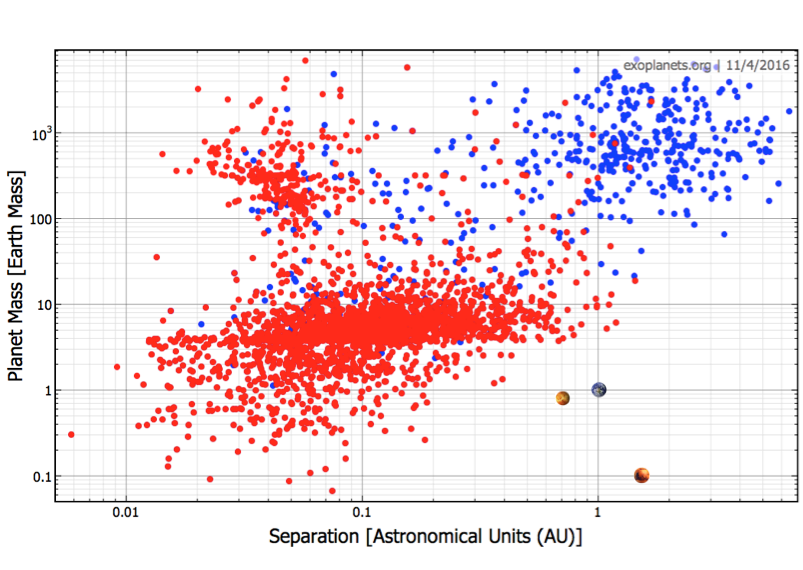
\includegraphics[width=0.8\textwidth]{exo_solar}
%\vspace{-0.5in}
\caption{Planetary mass vs. orbital separation of the detected exoplanet population, via transit (red) and radial velocity (blue). Venus, Mars and Earth are displayed in the lower right corner. The detected Super Earths have no Solar System analogs.}
\label{fig:chemical}
\end{figure}

\begin{figure}[h!]
\centering
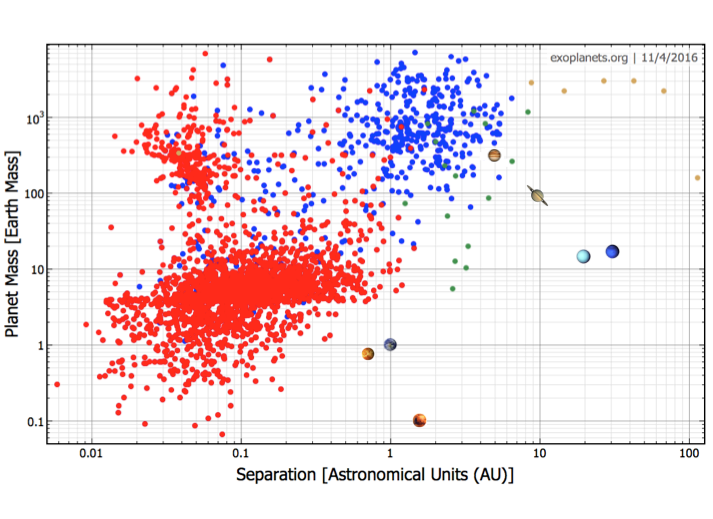
\includegraphics[width=0.8\textwidth]{exo_solar_all}
%\vspace{-0.5in}
\caption{Same as above, but planets detected via gravitational microlensing (green) and direct imaging (yellow) are added. Besides the terrestrial planets, Jupiter, Saturn, Uranus and Neptune are also shown. There is currently a scarcity of exoplanets with Earth to Saturn Masses outside $\sim$5 AU. New direct imaging surveys are expected to fill in this phase space.}
\label{fig:chemical}
\end{figure}

\vspace{0.2in}

%\section{Coupled Chemical and Dynamical Disk Evolution} 
\textbf{1. Planet formation from the start.} Planet formation models largely fall in two categories: core accretion, where planetesimals collide and grow into a solid core which then accretes a gaseous envelope, and gravitational instability, where planets form due to an instability in the disk that causes the disk material to collapse under its own gravity. Core accretion models can track a planet's mass, radius and luminosity evolution from the very early stages of its formation. Current core accretion models focus primarily on gas giants ([4], [5]), but no equivalent numerical simulations exist for lower mass planets. \textbf{Using the expertise that I acquired during my dissertation research on the evolution of gas giants (see Figure 3), I will use and improve the model I developed in [6] and [7], and adapt it to Super Earth Formation.} This will provide us with valuable insight into a forming planet's luminosity and other physical properties from the beginning of the accretion of the gaseous envelope until the gas disk dissipation.  


%this dynamical model  develop a (chemical models of increasing complexity) simplified time-dependent chemistry, 


\vspace{0.2in}
%\section{Planet and Planetesimal Migration}
\textbf{2. Spontaneous mass loss.} After the end of the planet formation process and gas disk dispersal, a planet can lose its envelope either due to irradiation from its host star (photoevaporation), or due to its own cooling. Atmospheric mass loss, as well as the planet's cooling and contraction, will decrease a planet's luminosity in time. Most atmospheric escape models focus on mass loss due to photoevaporation ([8], [9]). However, [10] use an analytic model to consider both types of mass loss, and find that the mass loss due to internal cooling happens on a much faster timescale than due to photoevaporation. This implies that the former process is likely to dominate the cooling, mass and luminosity evolution of very young planets, which are the focus of this project. \textbf{Through numerical and analytic calculations, I will incorporate a planet's mass loss due to internal cooling in my model, and use this to track the planet's luminosity after disk dissipation.} 

\begin{figure}[h]
\centering
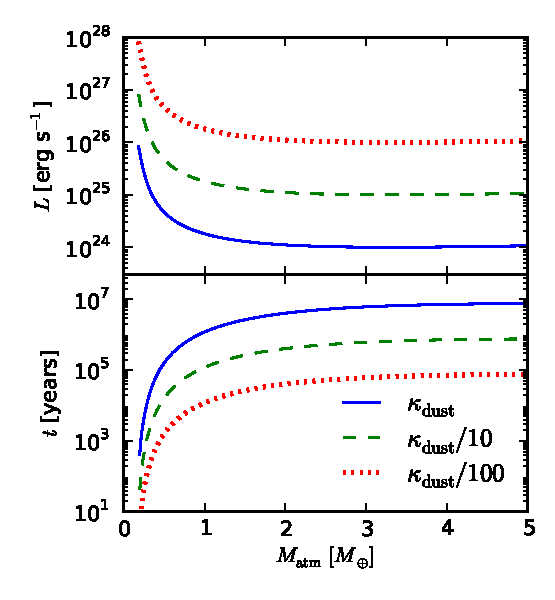
\includegraphics[width=0.5\textwidth]{opacity_effect.pdf}
%\vspace{-0.5in}
\caption{Example of a planet's luminosity and time evolution with atmospheric mass, during the giant planet formation stage. The different colored curves correspond to different assumptions about the atmospheric opacity. From [6].}  %The actual magnitude of dust opacities is difficult to robustly predict.}
\label{fig:LtvsMopacity}
\end{figure}

\vspace{0.2in}

%\section{Model Planet Populations} 
\textbf{3. Luminosity evolution and connection to observations.} A planet's luminosity evolution has been analyzed before [11], but this was only done for gas giants. Moreover, these models consider arbitrary initial conditions, as they are only interested in studying the luminosities of mature, several billion years old exoplanets. \textbf{The combined results from parts 1 and 2 will represent the first time that a planet's luminosity evolution is tracked self consistently from its birth through after the disk dispersal.} These results will be crucial for determining the masses of directly imaged exoplanets. They will be essential for correctly extrapolating from the observations of young, and hence bright systems, to the underlying population of exoplanets that is dominated by older, and hence significantly less luminous planets that will remain undetectable. Furthermore, these results may be able to help us distinguish between different formation scenarios --- core accretion versus gravitational instability. 

\vspace{0.2in}

\textbf{UCLA is the ideal place for me to continue my postdoctoral tenure as a President's Fellow.} I have tremendously enjoyed the time that I have spent here, and greatly benefitted from the diversity and academic excellence of the EPSS department. In particular, working with Prof. Hilke Schlichting is a privilege, and her expertise in planet formation and dynamics will be instrumental in achieving my research goals as a postdoctoral fellow and afterwards. Collaborating with Prof. David Jewitt, a leader in Solar System astrophysics, will be very useful for analyzing my findings in the context of the Solar System. As my research interests are at the intersection of astrophysics and planetary science, I would welcome collaborations with members of the Astronomy department faculty, such as Prof. Smadar Naoz. UCLA is also home to the Institute for Planets and Exoplanets (iPLEX), an interdisciplinary forum that ties together people with different scientific backgrounds. %Outside research, I plan to be involved in the UCLA Social Postdoc Society. Through this, I will help foster connections between postdoctoral scholars from various departments across the campus, with the goal of sharing our diverse scientific knowledge and experience.
%\begin{figure}[h!]
%\centering
%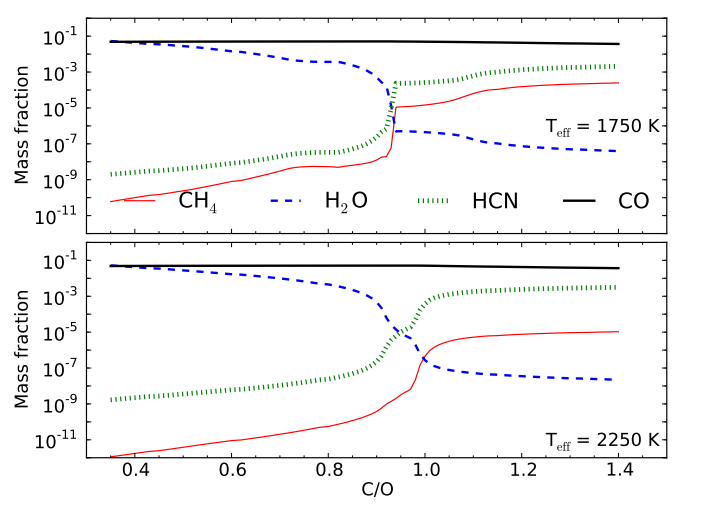
\includegraphics[width=0.7\textwidth]{CO_abundances}
%%\vspace{-0.5in}
%\caption{TBD}
%\label{fig:CO}
%\end{figure}




%\if\bibinc n
%\bibliography{refs}
%\fi
\FloatBarrier
%\def\bibfont{\footnotesize}
%\setlength{\bibsep}{0.0pt}

\section*{References}
\footnotesize
%\begin{thebibliography} {9}
\noindent $[1]$ Batalha, N. M. 2014, Proceedings of the National Academy of Science, 111, 12647 \\
$[2]$ Lissauer J. J., Dawson R. I., Tremaine S., 2014, Nature, 513, 336 \\
$[3]$ Fressin, F., Torres, G., Charbonneau, D., et al. 2013, ApJ, 766, 81\\
$[4]$ Pollack, J. B., Hubickyj, O., Bodenheimer, P., et al. 1996, Icarus, 124, 62 \\
$[5]$ Rafikov, R.R. 2006, ApJ, 648, 666 \\
$[6]$ \textbf{Piso, A.-M. A., \& Youdin, A. N. 2014, ApJ, 786, 21} \\
$[7]$ \textbf{Piso, A.-M. A., Youdin, A. N., \& Murray-Clay, R. A. 2015, ApJ, 800, 82} \\
$[8]$ Lopez, E. D., Fortney, J. J., \& Miller, N. 2012, ApJ, 761, 59 \\
$[9]$ Owen, J. E., \& Jackson, A. P. 2012, MNRAS, 425, 2931 \\
$[10]$ Ginzburg, S., Schlichting, H. E., \& Sari, R. 2016, ApJ, 825, 29 \\
$[11]$ Marley, M. S., Fortney, J. J., Hubickyj, O., Bodenheimer, P., \& Lissauer, J. J. 2007, ApJ, 655, 541



%\end{thebibliography}

%\bibliographystyle{abbrv}
%\bibliography{refs}


%\if\bibinc y
%\begin{thebibliography}
%\end{thebibliography}
%\fi


\end{document}